\documentclass[
	% -- opções da classe memoir --
	article,			% indica que é um artigo acadêmico
	11pt,				% tamanho da fonte
	oneside,			% para impressão apenas no recto. Oposto a twoside
	a4paper,			% tamanho do papel.
	% -- opções da classe abntex2 --
	%chapter=TITLE,		% títulos de capítulos convertidos em letras maiúsculas
	%section=TITLE,		% títulos de seções convertidos em letras maiúsculas
	%subsection=TITLE,	% títulos de subseções convertidos em letras maiúsculas
	%subsubsection=TITLE % títulos de subsubseções convertidos em letras maiúsculas
	% -- opções do pacote babel --
	english,			% idioma adicional para hifenização
	brazil,				% o último idioma é o principal do documento
	sumario=tradicional
	]{abntex2}


% ---
% PACOTES
% ---

% ---
% Pacotes fundamentais
% ---
\usepackage{lmodern}			% Usa a fonte Latin Modern
\usepackage[T1]{fontenc}		% Selecao de codigos de fonte.
\usepackage[utf8]{inputenc}		% Codificacao do documento (conversão automática dos acentos)
\usepackage{indentfirst}		% Indenta o primeiro parágrafo de cada seção.
\usepackage{nomencl} 			% Lista de simbolos
\usepackage{color}				% Controle das cores
\usepackage{graphicx}			% Inclusão de gráficos
\usepackage{microtype} 			% para melhorias de justificação
% ---
\usepackage{hyperref}
\usepackage{listings}
\usepackage{xcolor}
\usepackage{tcolorbox}
\usepackage{siunitx}
\usepackage{pdfpages}
% ---
% Pacotes adicionais, usados apenas no âmbito do Modelo Canônico do abnteX2
% ---
\usepackage{lipsum}				% para geração de dummy text
% ---

% ---
% Pacotes de citações
% ---
\usepackage[brazilian,hyperpageref]{backref}	 % Paginas com as citações na bibl
\usepackage[alf, abnt-emphasize=bf]{abntex2cite} % Estilo ABNT alfabético% ---

% ---
% Configurações do pacote backref
% Usado sem a opção hyperpageref de backref
\renewcommand{\backrefpagesname}{Citado na(s) página(s):~}
% Texto padrão antes do número das páginas
\renewcommand{\backref}{}
% Define os textos da citação
\renewcommand*{\backrefalt}[4]{
	\ifcase #1 %
		Nenhuma citação no texto.%
	\or
		Citado na página #2.%
	\else
		Citado #1 vezes nas páginas #2.%
	\fi}%
% ---

% --- Informações de dados para CAPA e FOLHA DE ROSTO ---
\titulo{ESTUDO E RESOLUÇÃO DO CICLO DE RANKINE COM MODIFICAÇÕES}
\tituloestrangeiro{}

\autor{
João Alex Arruda da Silva
\\[0.5cm]
Hanna Rodrigues Ferreira}

\local{Brasil}
\data{Fevereiro, 2025}
% ---

% ---
% Configurações de aparência do PDF final

% alterando o aspecto da cor azul
\definecolor{blue}{RGB}{41,5,195}

% informações do PDF
\makeatletter
\hypersetup{
     	%pagebackref=true,
		pdftitle={\@title},
		pdfauthor={\@author},
    	pdfsubject={Modelo de artigo científico com abnTeX2},
	    pdfcreator={LaTeX with abnTeX2},
		pdfkeywords={abnt}{latex}{abntex}{abntex2}{atigo científico},
		colorlinks=true,       		% false: boxed links; true: colored links
    	linkcolor=blue,          	% color of internal links
    	citecolor=blue,        		% color of links to bibliography
    	filecolor=magenta,      		% color of file links
		urlcolor=blue,
		bookmarksdepth=4
}
\makeatother
% ---

% ---
% compila o indice
% ---
\makeindex
% ---

% ---
% Altera as margens padrões
% ---
\setlrmarginsandblock{3cm}{3cm}{*}
\setulmarginsandblock{3cm}{3cm}{*}
\checkandfixthelayout
% ---

% ---
% Espaçamentos entre linhas e parágrafos
% ---

% O tamanho do parágrafo é dado por:
\setlength{\parindent}{1.3cm}

% Controle do espaçamento entre um parágrafo e outro:
\setlength{\parskip}{0.2cm}  % tente também \onelineskip

% Espaçamento simples
\SingleSpacing


% ----
% Início do documento
% ----
\begin{document}

% Seleciona o idioma do documento (conforme pacotes do babel)
%\selectlanguage{english}
\selectlanguage{brazil}

% Retira espaço extra obsoleto entre as frases.
\frenchspacing

% ----------------------------------------------------------
% ELEMENTOS PRÉ-TEXTUAIS
% ----------------------------------------------------------

%---
%
% Se desejar escrever o artigo em duas colunas, descomente a linha abaixo
% e a linha com o texto ``FIM DE ARTIGO EM DUAS COLUNAS''.
% \twocolumn[    		% INICIO DE ARTIGO EM DUAS COLUNAS
%
%---

% página de titulo principal (obrigatório)
\maketitle


% titulo em outro idioma (opcional)



% resumo em português
\begin{resumoumacoluna}
 Conforme a ABNT NBR 6022:2018, o resumo no idioma do documento é elemento obrigatório.
 Constituído de uma sequência de frases concisas e objetivas e não de uma
 simples enumeração de tópicos, não ultrapassando 250 palavras, seguido, logo
 abaixo, das palavras representativas do conteúdo do trabalho, isto é,
 palavras-chave e/ou descritores, conforme a NBR 6028. (\ldots) As
 palavras-chave devem figurar logo abaixo do resumo, antecedidas da expressão
 Palavras-chave:, separadas entre si por ponto e finalizadas também por ponto.

 \vspace{\onelineskip}

 \noindent
 \textbf{Palavras-chave}: latex. abntex. editoração de texto.
\end{resumoumacoluna}

% ----------------------------------------------------------
% ELEMENTOS TEXTUAIS
% ----------------------------------------------------------
\textual

% ----------------------------------------------------------
% Introdução
% ----------------------------------------------------------
\section{Introdução}

Segundo \cite{moran-2018}, o ciclo de Rankine é a estrutura fundamental das usinas termelétricas que operam com vapor. Este é um dos principais ciclos termodinâmicos utilizados na engenharia mecânica para conversão de calor em trabalho, sendo a base para o funcionamento de usinas termoelétricas e outras instalações de geração de energia. Esse ciclo opera com um fluido de trabalho, geralmente água, que passa por processos de aquecimento, expansão, resfriamento e compressão.

Para melhorar a eficiência do Ciclo de Rankine, diversas modificações são adotadas, como o superaquecimento, o reaquecimento e o uso de ciclos supercríticos. Essas modificações têm o objetivo de aumentar a eficiência térmica e reduzir perdas energéticas, tornando as plantas de geração mais sustentáveis e econômicas.

Este trabalho pretende analisar detalhadamente o ciclo de Rankine e suas variações, visando aprofundar o conhecimento sobre sistemas térmicos voltados à produção de energia. Para isso, será realizada uma revisão teórica robusta dos princípios termodinâmicos envolvidos, seguida da aplicação desses conceitos em um estudo de caso prático, que abordará técnicas como reaquecimento, expansão em dois estágios e regeneração térmica.

\section{Revisão bibliográfica}

\subsection{Definição do ciclo de Rankine}

O Ciclo de Rankine é um ciclo termodinâmico idealizado que descreve o funcionamento de uma usina termelétrica convencional. Esse ciclo é composto por quatro processos termodinâmicos: compressão, aquecimento, expansão e resfriamento. A Figura \ref{fig:esquema-simplificado-ciclo-rankine} ilustra o diagrama de um ciclo de Rankine básico.

\begin{figure}[h]
	\centering
	\caption{Esquema simplificado e o diagrama T-S do ciclo Rankine}
	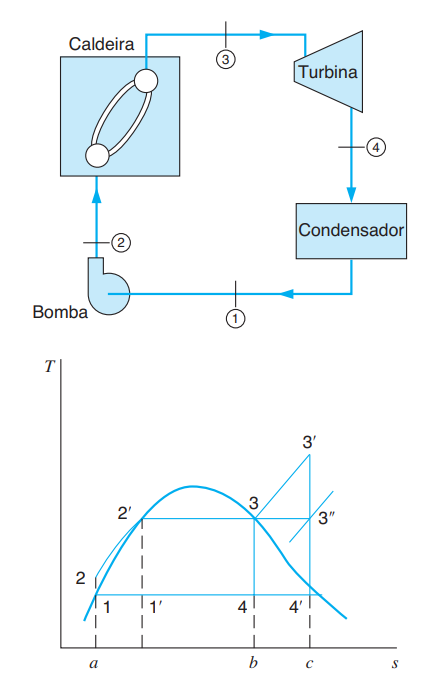
\includegraphics[width=0.7\textwidth]{./images/Esquema simplificado e o diagrama T-S do ciclo Rankine.png}
	\label{fig:esquema-simplificado-ciclo-rankine}
	\fonte{Adaptado de \cite{borgnakke-2020}}
\end{figure}

% ---
% Finaliza a parte no bookmark do PDF, para que se inicie o bookmark na raiz
% ---
\bookmarksetup{startatroot}%
% ---

% ---
% Conclusão
% ---
\section{Considerações finais}

% ----------------------------------------------------------
% ELEMENTOS PÓS-TEXTUAIS
% ----------------------------------------------------------
\postextual

% ----------------------------------------------------------
% Referências bibliográficas
% ----------------------------------------------------------
\bibliography{references}


\end{document}
